\title{PS2 Solutions}

%TEMPLATE HEADER
%This is the homework solution template
\documentclass[11pt]{article}

%AMS-TeX packages
\usepackage{amssymb, amsmath, amsthm} 
\usepackage[margin=.75in]{geometry}
\usepackage{graphicx}
\usepackage{caption}
\usepackage{subcaption}
\usepackage[utf8]{inputenc}
\usepackage{bm} % bold math
\usepackage{listings}
\usepackage{color} %red, green, blue, yellow, cyan, magenta, black, white
\definecolor{mygreen}{RGB}{28,172,0} % color values Red, Green, Blue
\definecolor{mylilas}{RGB}{170,55,241}

%Redefining sections as problems
\makeatletter 
\newenvironment{problem}{\@startsection
       {section}
       {1}
       {-.2em}
       {-3.5ex plus -1ex minus -.2ex}
       {0.2ex plus .2ex}
       {\pagebreak[3]%forces pagebreak when space is small; use \eject for better results
       \Large\sc\noindent{Problem }}\\}
\makeatother

%Fancy-header package to modify header/page numbering 
\usepackage{fancyhdr}
\pagestyle{fancy}
\lhead{\textbf{Ge/ESE 118}} %name of the course
\chead{\textbf{}} %topic of the homework set
\rhead{\textbf{Solution 2}} %number of the homework set
\lfoot{}
\cfoot{}
\rfoot{\thepage}

%Include frequently used commands used for equations
%Fractions
\newcommand\fr[2]{\frac{#1}{#2}} %Regular fraction

%Braces, Brackets, Parentheses, etc.
\newcommand\brcs[1]{\{#1\}} %Braces
\newcommand\brckts[1]{\left[#1\right]} %Brackets
\newcommand\lr[1]{\left(#1\right)} %Parentheses
\newcommand\abs[1]{\Big\lvert#1\Big\rvert} %Absolute value
\newcommand\ltwo[1]{\lVert#1\rVert_2} %L2-norm
\newcommand\linf[1]{\lVert#1\rVert_\infty} %L2-norm

%Linear algebra
\newcommand\tr[1]{\text{tr}\left( \mathbf{#1}\right)} %Trace
\renewcommand\det[1]{\text{det}\left( \mathbf{#1}\right)} %Determinant

%Trigonometric & special functions
\newcommand\sinb[1]{\, \sin\left(#1\right)} %Sine with parentheses: sin(x)
\newcommand\cosb[1]{\, \cos\left(#1\right)} %Cosine with parentheses: cos(x)
\newcommand\tanb[1]{\, \tan\left(#1\right)} %Tangent with parentheses: tan(x)
\newcommand\cotb[1]{\, \cot\left(#1\right)} %Cotangent with parentheses: cot(x)
\newcommand\sinc[1]{\, \text{sinc}\left(#1\right)} %Sinc function: sinc = sin(x)/x

%Calculus
\renewcommand\d[1]{\, \text{d}#1} %Differential for integrals
\newcommand\der[2]{\frac{\text{d}#1}{\text{d}#2}} %Ordinary derivate first order
\newcommand\dder[2]{\frac{\text{d}^2#1}{\text{d}#2^2}} %Ordinary derivate second order
\newcommand\od[3]{\frac{\text{d}^{#3}#1}{\text{d}#2^{#3}}} %Ordinary derivate any order
\newcommand\pder[2]{\frac{\partial#1}{\partial#2}} %Partial derivate first order
\newcommand\pdder[2]{\frac{\partial^2#1}{\partial#2^2}} %Partial derivate second order
\newcommand\pd[3]{\frac{\partial^{#3}#1}{\partial#2^{#3}}} %Partial derivative any order

%Fourier transform
\newcommand\ft[1]{\hat{#1}} %Fourier coefficient

%Probability theory, Statistics
\newcommand\ex[1]{\mathbb{E}\left[#1\right]} %Expectation
\newcommand\pr[1]{\mathbb{P}\left(#1\right)} %Probability
\newcommand\Var[1]{\text{Var}\left(#1\right)} %Variance
\newcommand\Cov[1]{\text{Cov}\left(#1\right)} %Covariance
\newcommand\one{\mathbf{1}} %Unity

%Miscellaneous 
\renewcommand\mod{\text{mod}} %Modulo

\begin{document}


\lstset{language=Matlab,%
	  %basicstyle=\color{red},
  breaklines=true,%
  morekeywords={matlab2tikz},
  keywordstyle=\color{blue},%
  morekeywords=[2]{1}, keywordstyle=[2]{\color{black}},
  identifierstyle=\color{black},%}
  stringstyle=\color{mylilas},
  commentstyle=\color{mygreen},%
  showstringspaces=false,%without this there will be a symbol in the places where there is a space
  numbers=left,%
  numberstyle={\tiny \color{black}},% size of the numbers
  numbersep=9pt, % this defines how far the numbers are from the text
  emph=[1]{for,end,break},emphstyle=[1]\color{red}, %some words to emphasise
													  %emph=[2]{word1,word2}, emphstyle=[2]{style},    
}

\subsection*{Problem 1 (graded by Dunzhu) - 40 points}
\subsubsection*{(a) 5 points}
$m = [t_s, x_s, y_s, z_s, v]^T$ are model parameters. It's nonlinear.
\subsubsection*{(b) 10 points}

using the notation in class, in this case
\begin{eqnarray*}
g_i(m) = t_s + \frac{\sqrt{(x_s-x_i)^2 + (y_s-y_i)^2 + (z_s-z_i)^2} }{v}
\end{eqnarray*}
note $x_i,y_i,z_i$ is some known constant, and $d_i = t_i$. 

then the matrix $\hat{G}$, and the residue vector $\gamma$
\begin{eqnarray*}
\hat{G}_{ik} & = & \frac{\partial g_i}{\partial m_k}  \\
\gamma & = & - G^T(d - g(m))
\end{eqnarray*}
then the Hessian
\begin{eqnarray*}
H & = & G^T G - \sum_i (d_i - g_i) Q_i 
\end{eqnarray*}

The least square solution will be 
\begin{eqnarray*}
m := m - H^{-1} \gamma 
\end{eqnarray*}


define
\begin{eqnarray*}
  R   & = &\sqrt{(x_s-x_i)^2 + (y_s-y_i)^2 + (z_s-z_i)^2} \\
  n_x & = & (x_s-x_i)/R \\
  n_y & = & (y_s-y_i)/R \\
  n_z & = & (z_s-z_i)/R \\
  e   & = & t_s + R/v - d_i
\end{eqnarray*}
note these quantity depends on $i$.

then 
\begin{eqnarray*}
  G(i,:) & = & 
  \left(
  \begin{array}{c}
	1 \\ 
	n_x/v \\
	n_y/v \\
	n_z/v \\
	-\frac{R}{v^2}
  \end{array}
  \right)^T\\
  \gamma_i & = & 
  e \left(
  \begin{array}{c}
	1 \\ 
	n_x/v \\
	n_y/v \\
	n_z/v \\
	-\frac{R}{v^2}
  \end{array}
  \right)  
\end{eqnarray*}

Hessian

\begin{eqnarray*}
  H & = & \sum_i
  \left(
  \begin{array}{ccccc}
	1 & n_x/v & n_y/v & n_z/v & -R/v^2 \\
	& \frac{1}{v} \left( \frac{1}{v} n_x^2 + \frac{e}{R}(1-n_x^2) \right)
	& \frac{1}{v} \left( \frac{1}{v} n_x n_y - \frac{e}{R}(n_x n_y) \right)
	& \frac{1}{v} \left( \frac{1}{v} n_x n_z - \frac{e}{R}(n_x n_z) \right)
	& \frac{-n_x}{v^2} \left( \frac{R}{v} + e \right) \\
	& 
	& \frac{1}{v} \left( \frac{1}{v} n_y^2 + \frac{e}{R}(1-n_y^2) \right)
	& \frac{1}{v} \left( \frac{1}{v} n_y n_z - \frac{e}{R}(n_y n_z) \right)
	& \frac{-n_y}{v^2} \left( \frac{R}{v} + e \right) \\
	& &
	& \frac{1}{v} \left( \frac{1}{v} n_z^2 + \frac{e}{R}(1-n_z^2) \right)
	& \frac{-n_z}{v^2} \left( \frac{R}{v} + e \right) \\
	symmetric  & & & &  \frac{R}{v^3} \left( \frac{R}{v} + 2 e \right )
  \end{array}
  \right)
\end{eqnarray*}

inexact Hessian 
\begin{eqnarray*}
  G^T G & = & \sum_i
  \left(
  \begin{array}{ccccc}
	1 & n_x/v & n_y/v & n_z/v & -R/v^2 \\
	& \frac{1}{v} \left( \frac{1}{v} n_x^2 +  \right)
	& \frac{1}{v} \left( \frac{1}{v} n_x n_y  \right)
	& \frac{1}{v} \left( \frac{1}{v} n_x n_z  \right)
	& \frac{-n_x}{v^2} \left( \frac{R}{v} \right) \\
	& 
	& \frac{1}{v} \left( \frac{1}{v} n_y^2 +  \right)
	& \frac{1}{v} \left( \frac{1}{v} n_y n_z  \right)
	& \frac{-n_y}{v^2} \left( \frac{R}{v} \right) \\
	& &
	& \frac{1}{v} \left( \frac{1}{v} n_z^2  \right)
	& \frac{-n_z}{v^2} \left( \frac{R}{v} \right) \\
	symmetric  & & & &  \frac{R}{v^3} \left( \frac{R}{v} \right )
  \end{array}
  \right)
\end{eqnarray*}
which is similar to the same as exact Hessian if $e=0$.

\subsubsection*{(c) 10 points}
\lstinputlisting{hw2p1_simple.m}

\clearpage
\subsubsection*{(d) 10 points}
The best model we get is
\begin{eqnarray*}
  m & = & 
  \left(
  \begin{array}{c}
      315.147372215551 \\
          30.3124982007349 \\
         -17.1481612373344 \\
          15.9867180697526 \\
          5.26992730665649 
  \end{array}
  \right) 
\end{eqnarray*}
with prediction error at six stations
\begin{eqnarray*}
  d_i - g_i & = & 
  \left(
  \begin{array}{c}
       -0.000967665303107879 \\
      -0.00257624919419186\\
       0.00285105963382648\\
      -0.00508794038000815\\
      0.000968216227079211\\
        0.0048125790164022
  \end{array}
  \right) 
\end{eqnarray*}

\subsubsection*{(e) 5 points}
 The scatter plot of earthquake location forms an elliptical shape, pointing to stations, this indicates the trade off between $x_s$ and $y_s$, in other words, the earthquake location in this case is well constrained within this azimuth with respect to station position. The color also indicates the trade off between $t_s$ and distance, if event are near, $t_s$ will be larger.
\begin{figure}
  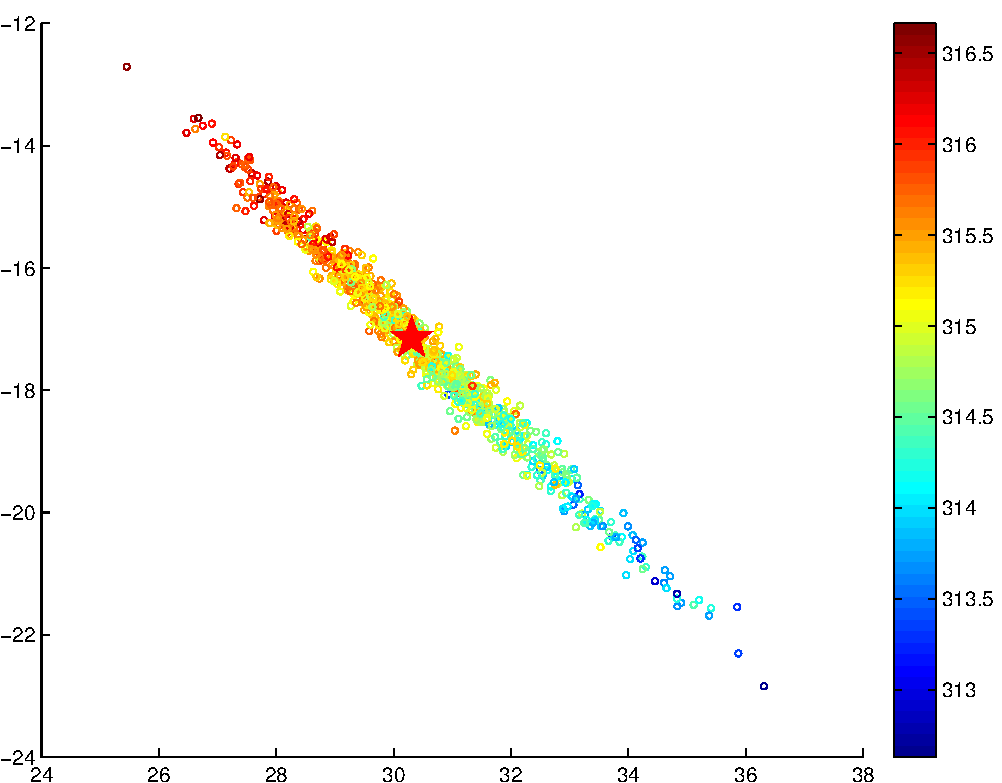
\includegraphics[width=8cm]{fig01.pdf}
  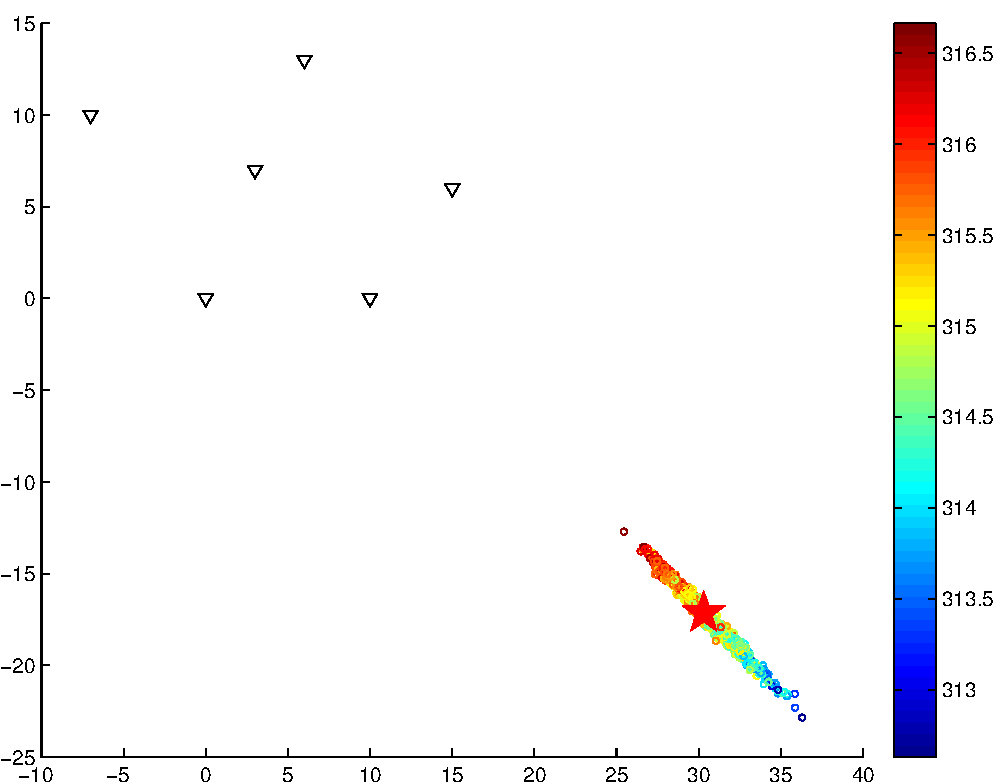
\includegraphics[width=8cm]{fig02.pdf}
  \caption{(e): Note the trade off between position and $t_s$. }
\end{figure}
\begin{figure}
\end{figure}

\newpage

\subsection*{Problem 2 (graded by Toby) - 15 points}
An example of a journal article that solves an inverse problem is \textit{Multiscale estimation of GPS velocity fields} by Carl Tape, Pablo Muse, Mark Simons, Danan Dong and Frank Webb. It was published in \textit{Geophysical Journal International} in 2009.

\subsubsection*{(a) - 5 points}
The data are velocity measurements from GPS stations. They are obtained at discrete locations. The authors mention the as reference frame error as a possible source of noise in their GPS data.

\subsection*{(b) - 5 points}
The model is the coefficients of a wavelet decomposition. The authors use a finite and discrete number of wavelets.

\subsection*{(c) - 5 points}
There are no ``physical laws'' that determine the operator $\mathbf{G}$ but it consists of the design matrix of the wavelet expansion. The operator is nonlinear in the locations, but linear in the model parameters. The authors discuss issues associtated with uniqueness and stability and they apply a regularization procedure to their least squares inversion.

\newpage

\subsection*{Problem 3 (graded by Stephen) - 45 points}
\subsubsection*{(a) 2 points}
(see Figure 1 below for plot)
\begin{figure}[htbp]
	\centerline{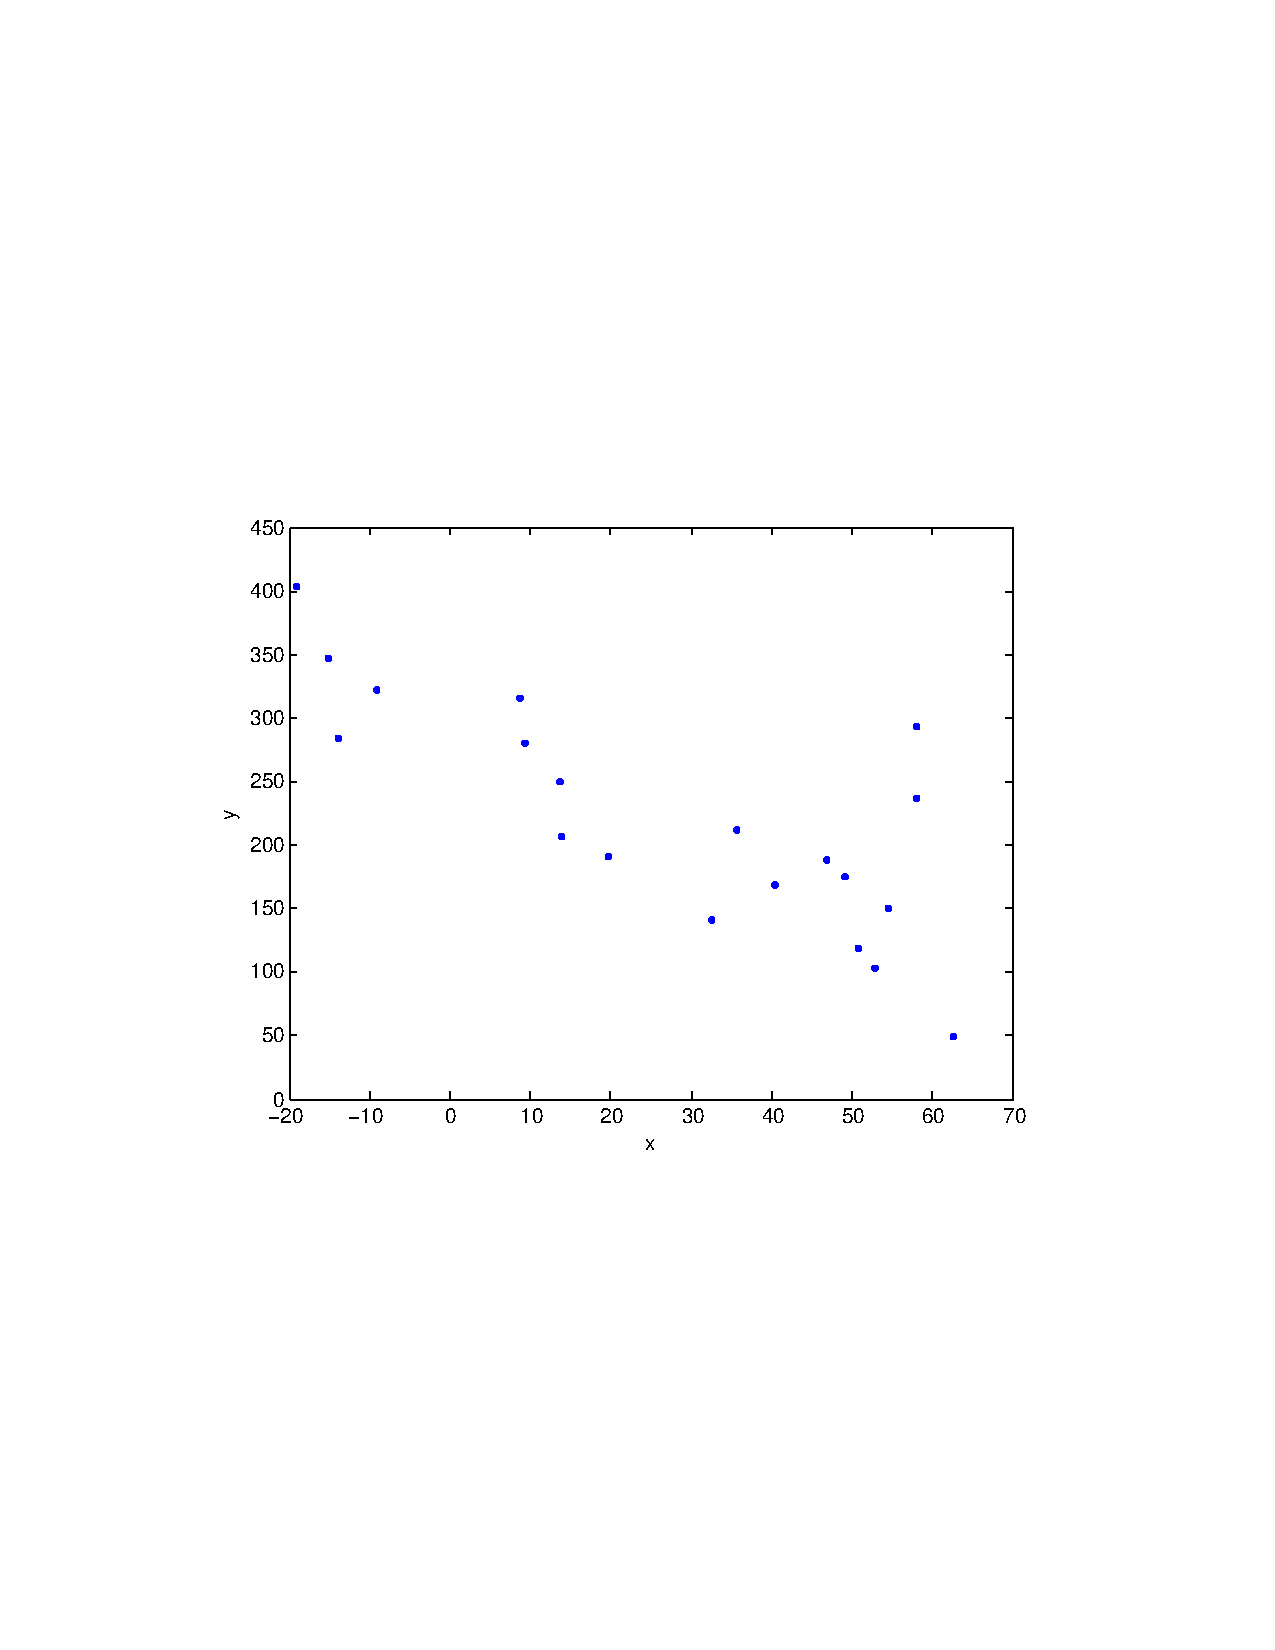
\includegraphics[width=1\textwidth]{Plot_Data.pdf}}
	\caption{\label{p1}%
	Data plotted for part a}
\end{figure}

\subsubsection*{(b) 3 points}
m1 = [100:0.1:500];
m2 = [-9:0.01:3];
The ranges can vary slightly as long as they have reasonable values.  We can get these estimates by looking at the plot and estimating slope and intercepts.  However, we need a conservative enough range that we don't have parts of the interesting region get cut off our later plots.

\subsubsection*{(c) 10 points}
\begin{verbatim}
function [misfit] = lineMisfit(type,x,y,m1,m2)
%type is either 1(L1) or 2(L2) norms
%x and y are the data we are using
%y = m1 + m2*x
%m1 is slope for linear fit and m2 is y-intercept


misfit = zeros(length(m1),length(m2));

if (type==1)        %do L1 misfit
    for(i=1:length(m1))
        for(j=1:length(m2))
            for(k=1:length(x))
                pointMisfit = abs(y(k) - (m1(i)+m2(j)*x(k)));
                misfit(i,j) = misfit(i,j) + pointMisfit;
            end
        end
    end
end

if (type==2)        %do L2 misfit
    for(i=1:length(m1))
        for(j=1:length(m2))
            for(k=1:length(x))
                pointMisfit = (y(k) - (m1(i)+m2(j)*x(k)))*((y(k) - (m1(i)+m2(j)*x(k))));
                misfit(i,j) = misfit(i,j) + pointMisfit;
            end
        end
    end
end
\end{verbatim}

\subsubsection*{(d) 10 points}
\begin{verbatim}
%L1 misfit
misfit = lineMisfit(1,x,y,m1,m2);

minmisfit = min(min(misfit));
maxmisfit = max(max(misfit));

figure;
pcolor(m2,m1,misfit)
xlabel('m2')
ylabel('m1')
shading flat
caxis([minmisfit minmisfit+0.15*(maxmisfit-minmisfit)])
hcb = colorbar;
colorTitleHandle = get(hcb,'Title');
titleString = 'L1 Misfit';
set(colorTitleHandle ,'String',titleString);


%L2 misfit
misfit2 = lineMisfit(2,x,y,m1,m2);

minmisfit2 = min(min(misfit2));
maxmisfit2 = max(max(misfit2));

figure;
pcolor(m2,m1,misfit2)
xlabel('m2')
ylabel('m1')
shading flat
caxis([minmisfit2 minmisfit2+0.15*(maxmisfit2-minmisfit2)])
hcb = colorbar;
colorTitleHandle = get(hcb,'Title');
titleString = 'L2 Misfit';
set(colorTitleHandle ,'String',titleString);
\end{verbatim}

(see below Figures 2 and 3 for output)

\begin{figure}[htbp]
	\centerline{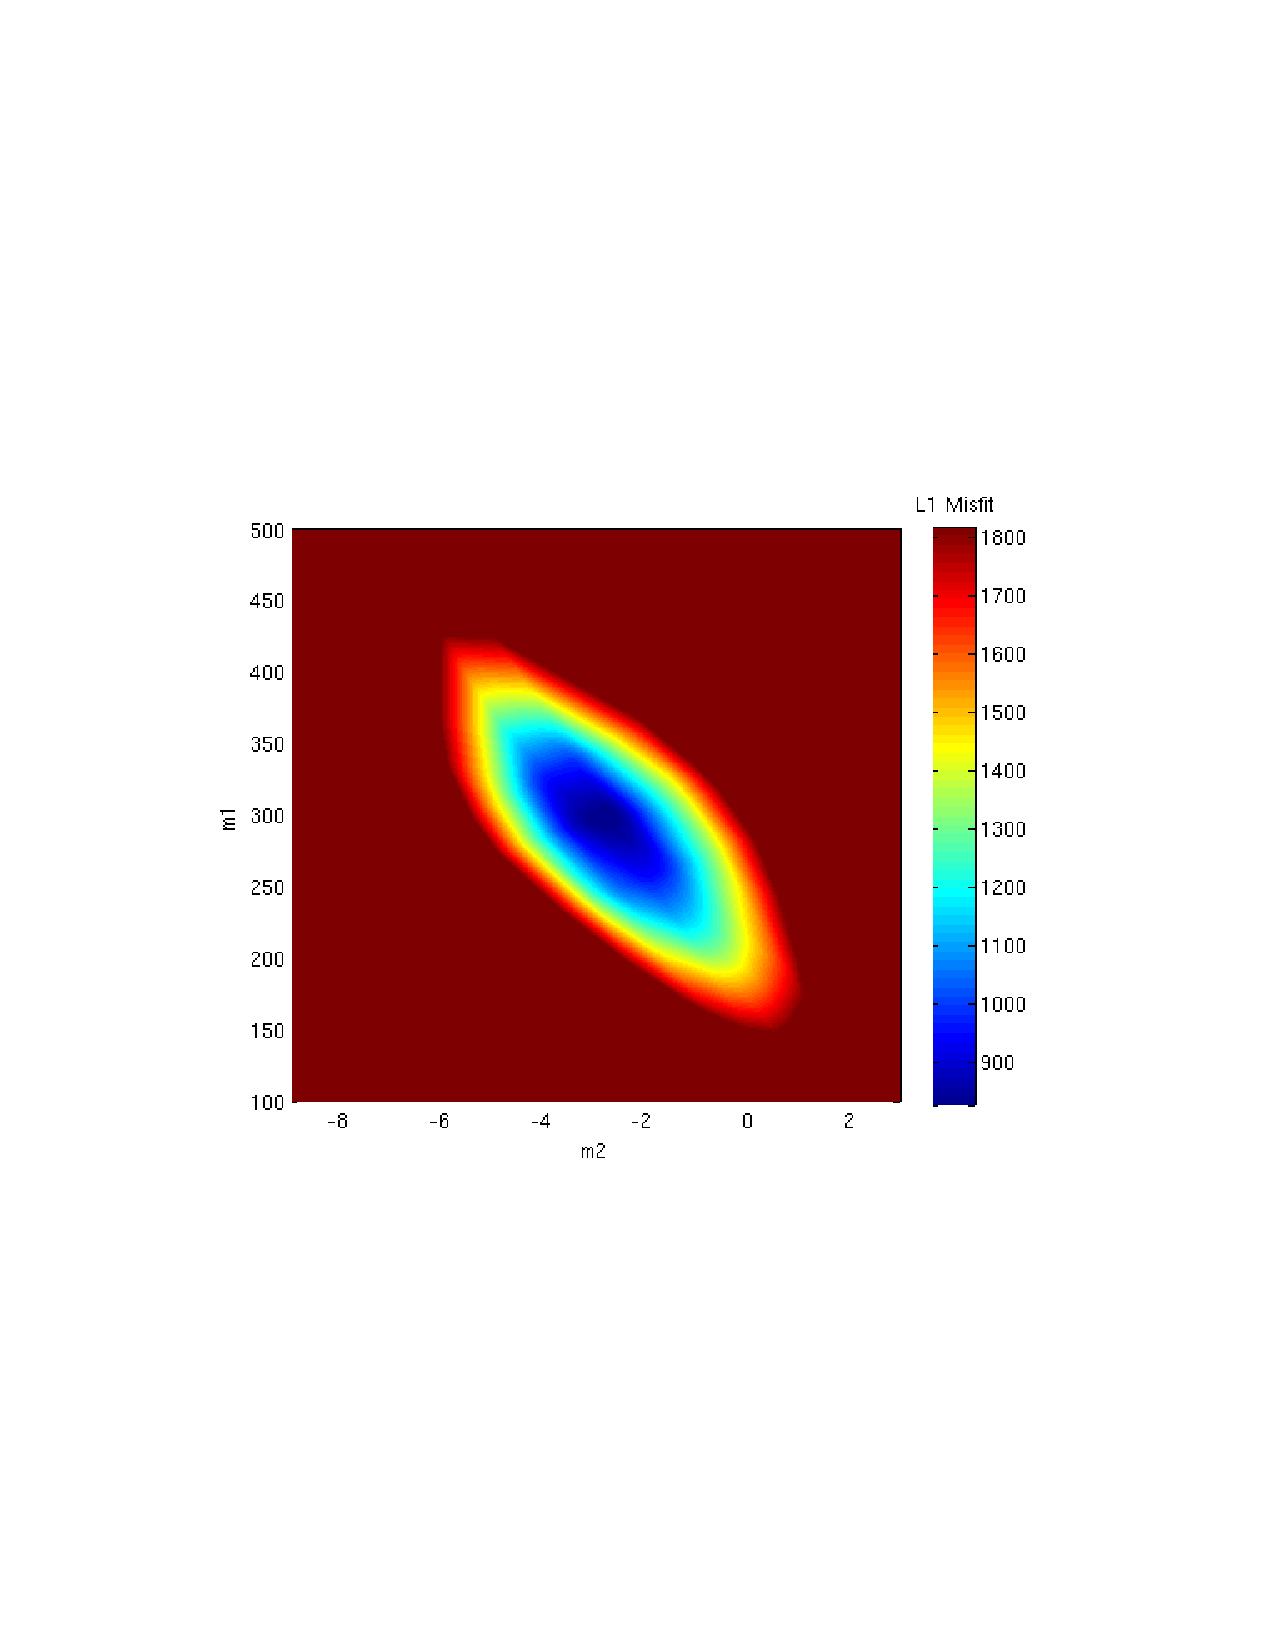
\includegraphics[width=1\textwidth]{L1Misfits.pdf}}
	\caption{\label{p1}%
	L1 misfits calculated for the whole relevant parameter space of m1 and m2.  Lower values (blue) are a better fit with the data.  We want a big enough range to see the entire interesting region.}
\end{figure}

\begin{figure}[htbp]
	\centerline{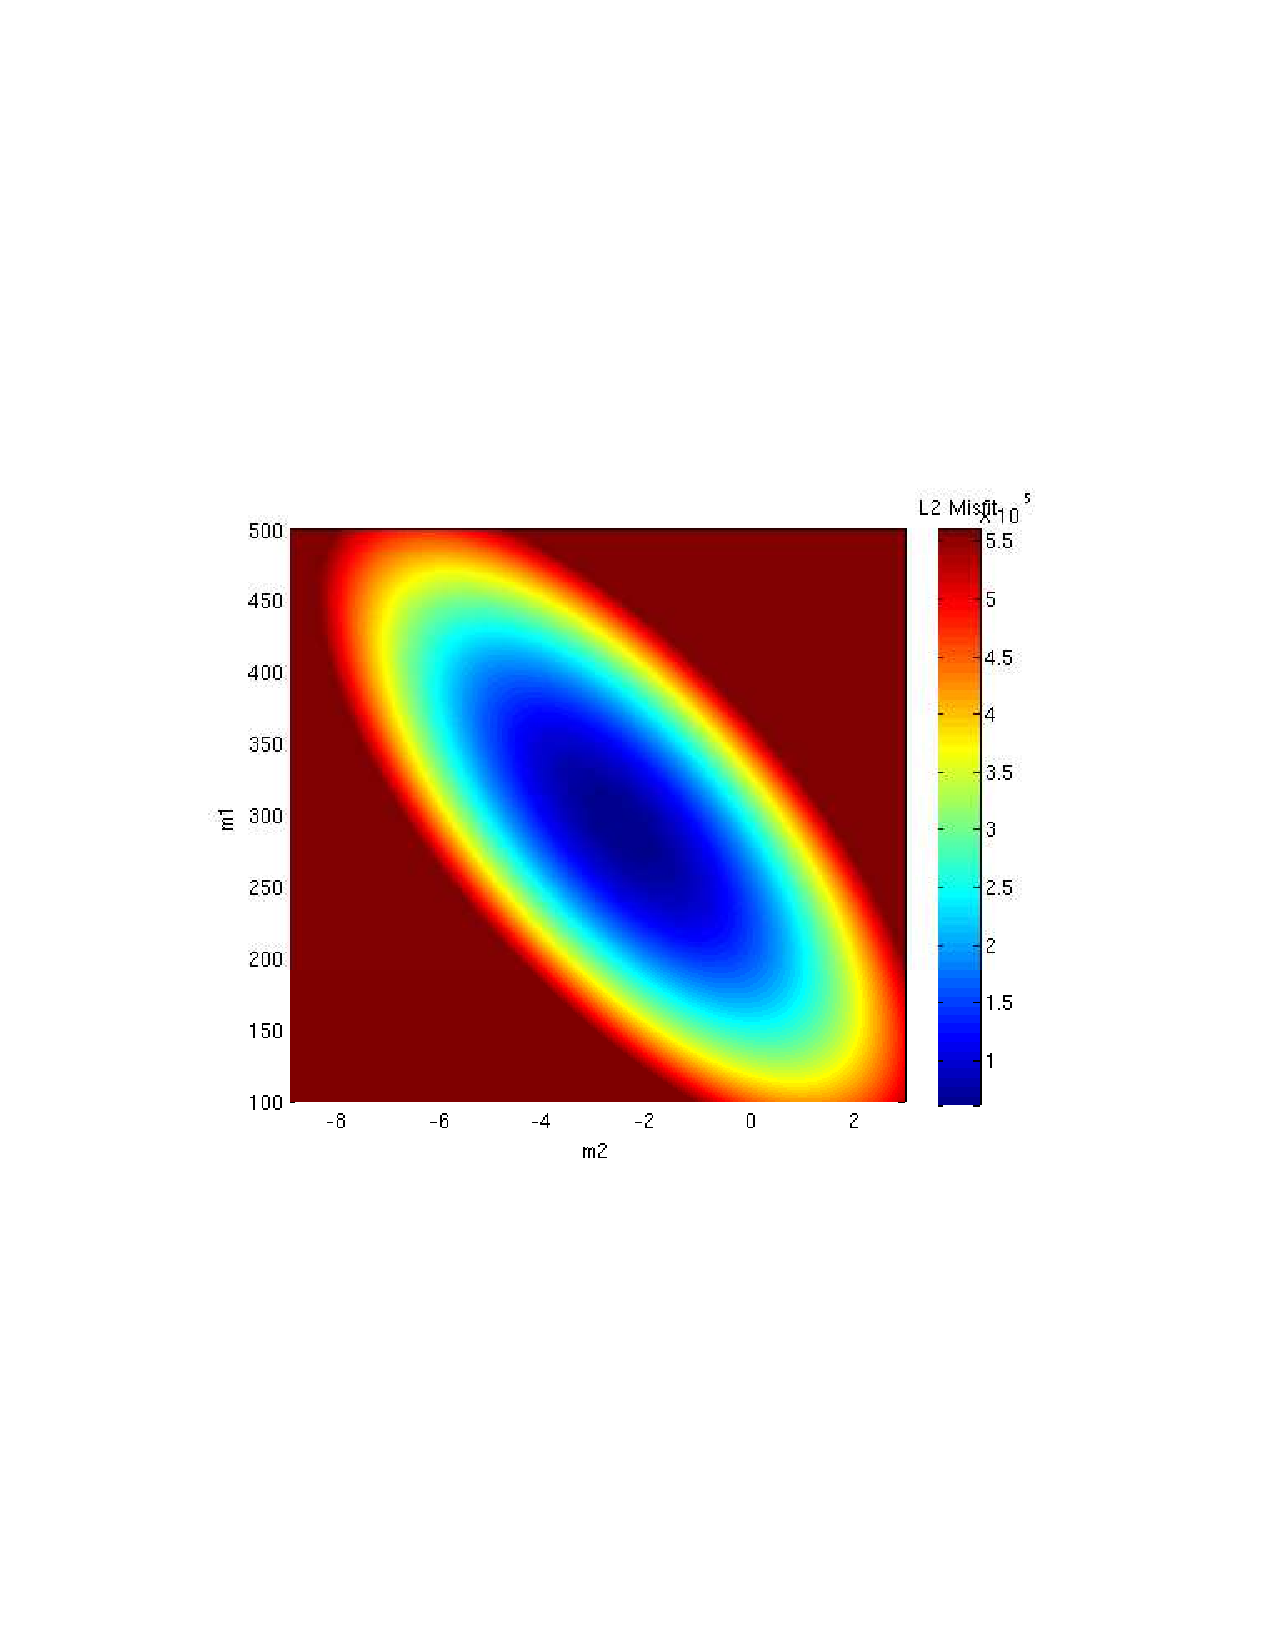
\includegraphics[width=1\textwidth]{L2Misfits.pdf}}
	\caption{\label{p1}%
	L2 misfits calculated for the whole relevant parameter space of m1 and m2.  Lower values (blue) are a better fit with the data.  This should have a big enough range to see the entire interesting region.}
\end{figure}

\subsubsection*{(e) 5 points}
\begin{verbatim}
[r1,c1]=find(misfit==min(min(misfit)));
[r2,c2]=find(misfit2==min(min(misfit2)));

L1bestm1=m1(r1)
L1bestm2=m2(c1)
L2bestm1=m1(r2)
L2bestm2=m2(c2)
\end{verbatim}

Answers will vary slightly depending on the resolution of the discretization.  For my ranges of $m_1$ and $m_2$ above I get the following values:
L1: $m_1 = 297.2$, $m_2 = -2.7$
L2: $m_1 = 292$, $m_2 = -2.55$

\subsubsection*{(f) 5 points}
Formula for finding the best fit for method of least squares:
$m_{LLS} = (G^{T}G)^{-1}G^{T}d$

\begin{verbatim}
G = [ones(20,1) x];          %we get this from our m1+m2*x
%now plug into our formula
m = (G'*G)^-1*G'*y
\end{verbatim}

This should give $m_1 = 291.8387$ and $m_2 = -2.5454$ as the exact LLS solution.

\subsubsection*{(g) 5 points}
The plots produced in d show a great deal of information about the whole
model space that is only summarized in a standard result.  The standard
result shows the best fit parameters and the standard deviation, but it
doesn't show any correlation between the parameters.  It's not as useful
because we can't see the region of good fit in a realistic model space; we
can only see what the exact best fits are.

\subsubsection*{(h) 5 points}
Will take any answer as correct as long as it's well defended.  The L1 and
L2 would be preferred because they are more descriptive of the model space
and we can see what realistic model values would give low misfits.  Least
squares does not show this level of description.  However, it is not
discretized and instead gives the exact answer.  It's also faster and less
computationally expensive which could be important in real research
questions.

Different error bars shouldn't change the answer much, but if we have some
significant outliers then L1 would be preferable to L2.  This is due to the fact that the L1 norm is more robust than the L2 norm because it doesn't weight outliers as much.  For L1, the absolute value of the error matters, whereas for L2 we look at the square of the error.  In the case of an outlier, the squared error will be much larger than the absolute value.

If the error bars are large then we can say some of
the misfit can be explained by measurement error.  However, in this case
the error bars are small compared to the data scatter, so measurement
error is not a significant source of misfit.




\end{document}